\documentclass{beamer}

\usetheme{Warsaw}
\usepackage{multirow}
\title{Introduction to ANN, DTrees and Clustering}

\author{Khaled El-Wazan \thanks{khaled\_elwazan@alex-sci.edu.eg}}

\institute{Department of Mathematics and Computer Science, Faculty of Science, Alexandria University}

\date{}

\AtBeginSection[]{
  \begin{frame}
  \vfill
  \centering
  \begin{beamercolorbox}[sep=8pt,center,shadow=true,rounded=true]{title}
    \usebeamerfont{title} \thesection: \insertsectionhead\par%
  \end{beamercolorbox}
  \vfill
  \end{frame}
}

\setbeamertemplate{caption}[numbered]

% remove headlines at a certain frame

\makeatletter
    \newenvironment{withoutheadline}{
        \setbeamertemplate{headline}[default]
        \def\beamer@entrycode{\vspace*{-\headheight}}
    }{}
\makeatother

\begin{document}
\maketitle


\begin{frame}
	\frametitle{Outlines}
	
	\tableofcontents
	
	    
	
\end{frame}


\section{Artificial Neural Networks}


\subsection{Introduction}
\begin{frame}
	\frametitle{Introduction}
	Roots of work on neural Networks (NN) are from:
	\begin{itemize}
		\item  Neuro-biological studies (more than a century), e.g. how nerves behave when stimulated by different electric currents.
		\item Psychological studies, e.g. how animal learn, forget and recognize types and tasks.
		\item Psycho-physical experiments, and
		\item MaCulloch and Pitts, when they introduced their first mathematical model for single neurons.
	\end{itemize}   
	
\end{frame}


\begin{frame}
    \frametitle{Applications}

    \begin{itemize}
        \item Classification
        \begin{itemize}
            \item Image recognition
            \item Speech recognition
            \item Diagnostics
            \item Fraud detection
        \end{itemize}
        \item Regression
        \begin{itemize}
            \item Forecasting and prediction
        \end{itemize}
        \item Pattern association
        \begin{itemize}
            \item Retrieve an image from corrupted one
        \end{itemize}
        \item Clustering
        \begin{itemize}
            \item Client profiling
            \item Disease subtypes
        \end{itemize}
    \end{itemize}

\end{frame}


\begin{frame}
    \frametitle{Real Neural Learning}

    \begin{itemize}
        \item Synapsis change size and strength with experience.
        \item When $2$ connected neurons are firing at the same time, the strength of the synapse between them increase, i.e. Hebbian Learning.
        \item \textit{"Neurons that fire together, wire together." }
    \end{itemize}


\end{frame}


\begin{frame}
    \frametitle{Neural Network}

    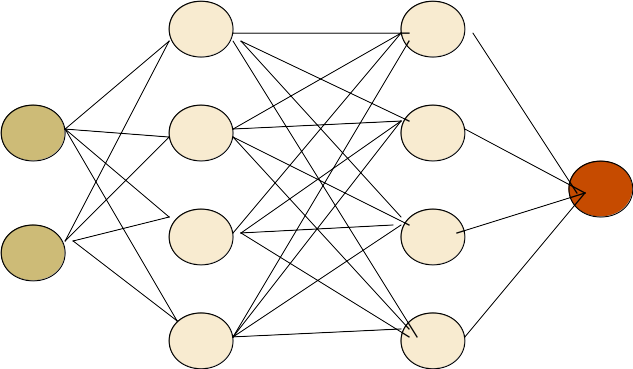
\includegraphics[width=\textwidth,height=\textheight,keepaspectratio]{assets/images/NN.png}
\end{frame}


\subsection{Single Artificial Neuron}

\begin{frame}
    \frametitle{Simple Aritifial Neuron}
    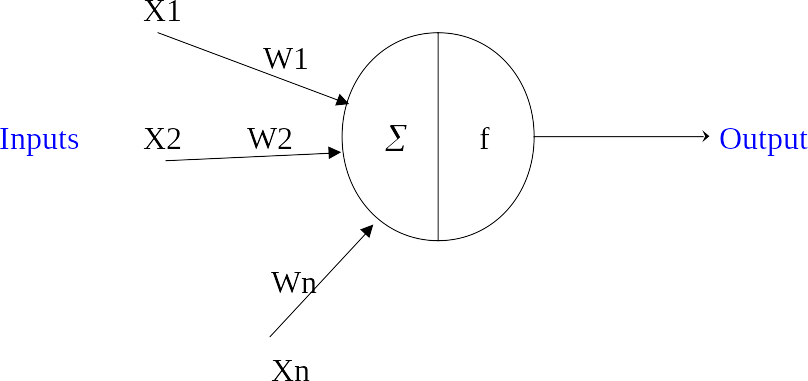
\includegraphics[width=\textwidth,height=\textheight,keepaspectratio]{assets/images/ANN.png}
\end{frame}


\begin{frame}
    \frametitle{Neuron Model}

    \begin{itemize}
        \item A neuron has more than one input, $x_1,x_2,\cdots, x_n$.
        \item Each input is associated with a weight $w_1,w_2,\cdots,w_n$.
        \item The neuron has a bias $b$.
        \item The net input of the neuron is calculated as follows:
        \begin{equation}
            z=\sum_{i=1}^n w_ix_i+b
        \end{equation}
        \item The neuron output is 
        \begin{equation}
            y=f(z),    
        \end{equation}
        where $f$ is called \textbf{transfer function}.
    \end{itemize}
\end{frame}


\begin{frame}
    \frametitle{Transfer Function}
    We have $3$ common transfer functions:
    \begin{itemize}
        \item Hard limit transfer function
        
       \begin{equation}
        y=f(z)=
        \begin{cases}
          1, & z \ge \tau\\
          0, & \text{otherwise}
        \end{cases},
       \end{equation}
       where $\tau$ is a certain desired threshold.

        \item Linear transfer function,
        \begin{equation}
            y=f(z)=a\times z+b,
        \end{equation}
        where $a$ and $b$ are constants, and
        \item Sigmoid transfer function
        \begin{equation}
            f(z)=\frac{1}{1+e^{-z}}.
        \end{equation}
    \end{itemize}

\end{frame}


\begin{frame}
    \frametitle{Architecture of ANN}
        \begin{itemize}
            \item \textit{Feed-forward network.} Allow the signals to travel one way from the input layer to the output layer, in case of multilayer ANN.
            \item \textit{Feed-back networks.} The signal travels as loops in the network, the output is connected to the input of the network.    
       
        \end{itemize}


    

\end{frame}


\begin{frame}
    \frametitle{Perceptron}
\begin{figure}[]
    \centering
    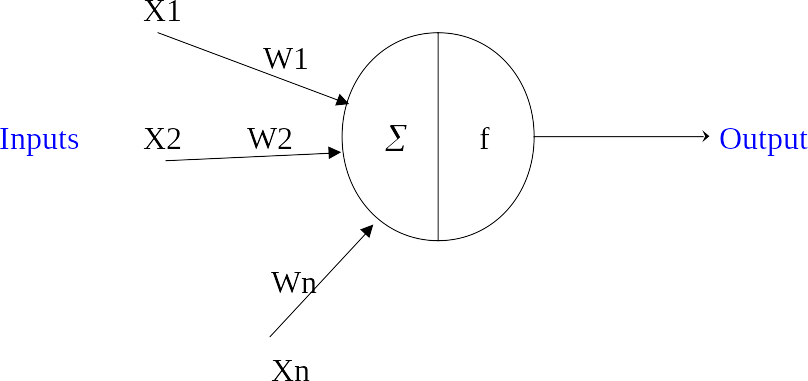
\includegraphics[width=\textwidth,height=\textheight,keepaspectratio]{assets/images/ANN.png}
    \caption{ It is a network of one neuron and hard limit transfer function}
\end{figure}

\end{frame}


\begin{frame}
    \frametitle{Perceptron Learning Rule}

    \begin{equation}
        W_{new}=W_{old}+(t-a)X,
    \end{equation}
where $W_{new}$ is the new weight, \\ $W_{old}$ is the old value of the weight,\\ $X$ is the input value, \\ $t$ is the desired output, and \\ $a$ is the actual value of the output.

\end{frame}


\begin{frame}
    \frametitle{Perceptron Example}
    \begin{figure}[]
        \centering
        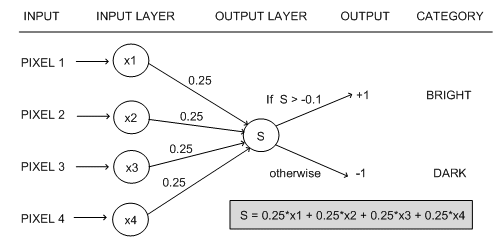
\includegraphics[width=\textwidth,height=\textheight,keepaspectratio]{assets/images/example.png}
        \caption{ A perceptron working example, categorizing image to either: \textit{bright} or \textit{black}.}
    \end{figure}
    
\end{frame}


\subsection{Multilayered ANN}

\begin{frame}[allowframebreaks]
    \frametitle{Learning Rule}

    \begin{itemize}
        \item The perceptron learning rule can not be applied to multi-layer network, so we use back propagation algorithm for the learning process.
    

    \begin{figure}[]
        \centering
        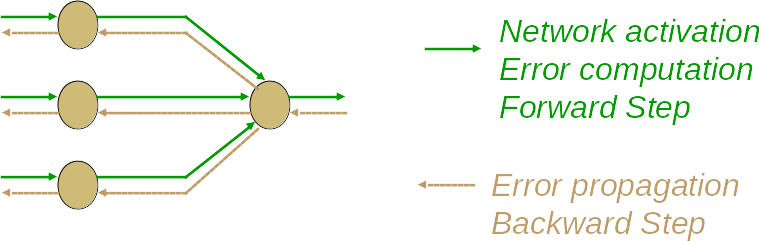
\includegraphics[width=\textwidth,height=\textheight,keepaspectratio]{assets/images/ann-bp.png}
        \caption{The wights are adjusted to minimize the mean squared error.}
    \end{figure}

    \item The weight change rule is:
    \begin{equation}
        \omega_{ij}^{new} = \omega_{ij}^{old}+\alpha\times \text{error}\times f^{'} (\text{input}),
    \end{equation}
where $\alpha$ is the learning factor, \\ $error$ the the difference between the actual data and the trained data, and \\
$f^{'}$ is the derivative of sigmoid function.

\end{itemize}

\end{frame}


\subsection{Building ANN}

\begin{frame}
    \frametitle{Building ANN}

How to build an ANN:

\begin{enumerate}
    \item \textit{Define the problem in terms of neurons.} Think in terms of the layers.
    \item \textit{Represent the information as neurons.} Operationalize neurons, select their data types and locate data for testing and learning.
    \item \textit{Define the network.}
    \item \textit{Train the network.}
    \item \textit{Test the network}
\end{enumerate}

\end{frame}




\section{Decision Trees}

\subsection{Introduction}

\begin{frame}
    \frametitle{Descision Trees}

What is a decision tree?

    \begin{itemize}
        \item A flow-chart-like tree structure.
        \item Internal nodes denotes an attribute
        \item Branch represents the values of the node attributes.
        \item Leaf nodes represent class labels or class distribution.
    \end{itemize}   

\end{frame}


\begin{frame}
    
    \begin{figure}[]
        \centering
        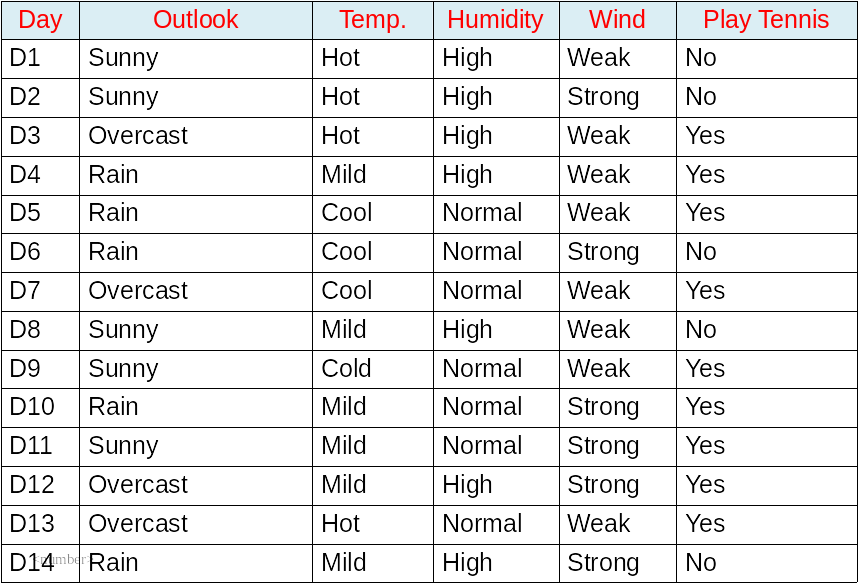
\includegraphics[width=75mm,height=75mm,keepaspectratio]{assets/images/Untitled.png}
        \caption{A table represent decisions based on certain attributes.}
        \label{fig:data_table}
    \end{figure}
\end{frame}


\begin{frame}
        
    \begin{figure}[]
        \centering
        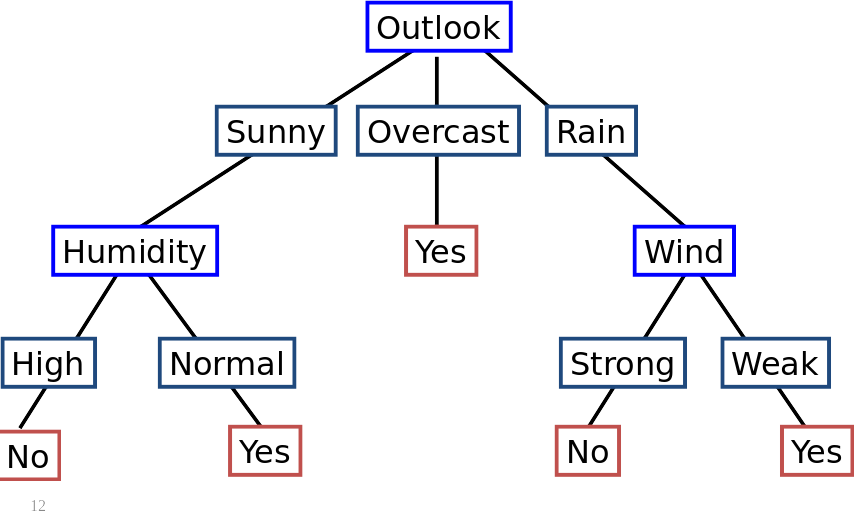
\includegraphics[width=\textwidth,height=\textheight,keepaspectratio]{assets/images/tree.png}
        \caption{A decision tree based on the given data provided in Figure ~\ref{fig:data_table}. }
    \end{figure}
\end{frame}

\subsection{Building a Decision Tree}

\begin{frame}
    \frametitle{Information Gain}

$Gain(S,A):$ expected reduction in entropy due to sorting $S$ on attribute $A$.

\begin{equation}
    Gain(S,A)=entropy(S)-\sum_{v\in values(A)}\frac{\vert S_v\vert }{\vert S\vert} entropy(S_v).
\end{equation}


\end{frame}


\begin{frame}[allowframebreaks]
    \frametitle{}

    \begin{figure}[]
        \centering
        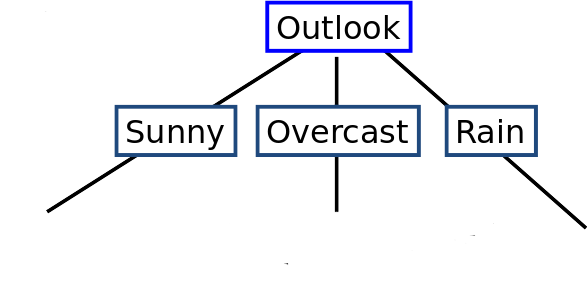
\includegraphics[width=60mm,height=60mm,keepaspectratio]{assets/images/step1.png}
        \caption{First step i building a decision tree: testing attributes and entropy.}
        \label{}
    \end{figure}

\begin{align*}
    Gain(S_{sunny, Humidity})&=0.97 \\
    Gain(S_{sunny},Temp)&=0.57 \\
    Gain(S_{sunny},Wind)&=0.019
\end{align*}

\begin{figure}[]
    \centering
    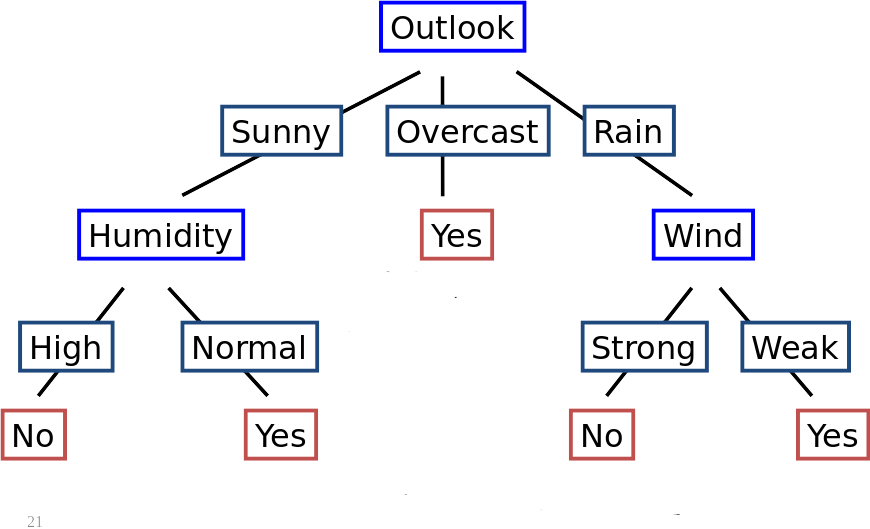
\includegraphics[width=\textwidth,height=\textheight,keepaspectratio]{assets/images/fulltree.png}
    \caption{The full tree of the given example.}
    \label{}
\end{figure}

\end{frame}



\begin{frame}
    \frametitle{Converting a Tree to Rules}
    \begin{figure}
        \centering
        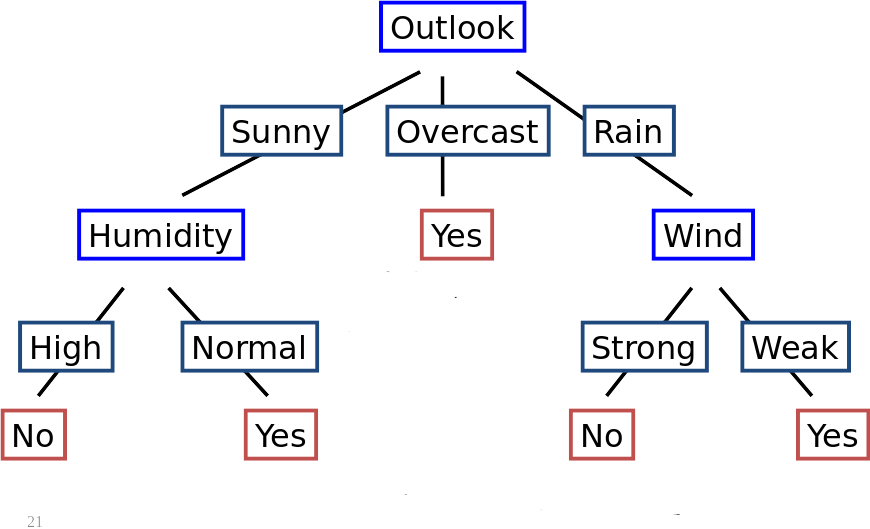
\includegraphics[width=40mm,height=40mm,keepaspectratio]{assets/images/fulltree.png}
    \end{figure}
    
    \begin{itemize}
        \item if(Outlook=Sunny) and (Humidity=High), then PlayTennis=No
        \item if(Outlook=Sunny) and (Humidity=Normal), then PlayTennis=Yes
        \item if(Outlook=Overcast), then PlayTennis=Yes
        \item if(Outlook=Rain) and (Wind=Strong), then PlayTennis=Normal
        \item if(Outlook=Rain) and (Wind=Weak), then PlayTennis=Yes 
    \end{itemize}

\end{frame}

\section{Clustering Analysis}


\subsection{Definition}

\begin{frame}
    \frametitle{Definition}

\begin{itemize}
    \item     Clustering is the task of grouping a set of objects such that all the collected object together are similar.
    \item Clustering techniques is applied when prediction classes are no defined or known.
    \item Unsupervised learning.
\end{itemize}
    

\end{frame}


\subsection{Algorithms}

\begin{frame}
    \frametitle{Algorithms}

There are several clustering algorithm which can be \textit{"clustered"} together based on their model, e.g.

\begin{itemize}
    \item Centroid-base,
    \item Grid-based,
    \item Denisty-based,
    \item Distribution-based, and
    \item Connectivity-based
\end{itemize}
    

\end{frame}



\begin{frame}[allowframebreaks]
    \frametitle{Centroid-based algorithm ($k$-means)}

The algorithm is carried as follows:

    \begin{enumerate}
        \item Partition objects into $k$ nonempty subsets
        \item \label{step}Compute seed points as the centroids of the clusters of the current partitioning (the centroid is the center, i.e., mean point, of the cluster)
        \item Assign each object to the cluster with the nearest seed point
        \item Go back to Step ~\ref{step}, stop when the assignment does not change.
    \end{enumerate}



\end{frame}


\section{Measuring the Performance of a Classifier}






\subsection{Confusion Matrix}


\begin{frame}

    \frametitle{Confusion Matrix}

    \begin{table}[h]
        \centering
                \begin{tabular}{l|lll}
                    \hline
                                         & \multicolumn{3}{c}{Predicted data}  \\\cline{2-4}
                                            & &$+$ & $-$        \\\hline
                     \multirow{2}{*}{Actual data}& $+$&\multicolumn{1}{l}{TP} & \multicolumn{1}{l}{FN} \\\cline{2-4}
                                       & $-$ & \multicolumn{1}{l}{FP} & \multicolumn{1}{l}{TN} \\\hline
                \end{tabular}
        \end{table}


    \begin{itemize}
        \item \textit{True positive (TP).} The number of positive instances that are classified as positive.
        \item \textit{False positive (FP).} The number of negative instances that are classified as positive.
        \item \textit{False negative (FN).} The number of positive instances that are classified as negative.
        \item \textit{True negative (TN).} The number of negative instances that are classified as negative.
    \end{itemize}
    

\end{frame}

\subsection{Types of Errors}

\begin{frame}
    \frametitle{Types of Errors}


    \begin{itemize}
        \item \textit{False positive.} Occurs when instances that should be classified as negative are classified as positive.
        \item \textit{False negative.} Occurs when instances that should be classified as positive are classified as negative.
    \end{itemize}
    

\end{frame}


\begin{frame}
    \frametitle{Summary}

\tableofcontents


\end{frame}


\begin{frame}

    \begin{center}
        \Huge Questions?
    \end{center}

\end{frame}

\end{document}
